\documentclass[a4paper, notitlepage]{report}
\newcommand{\Lim}[1]{\raisebox{0.5ex}{\scalebox{0.8}{$\displaystyle \lim_{#1}\;$}}}
\usepackage{amsmath, amsfonts, amsthm, amssymb}
\usepackage[margin=0.6in]{geometry}
\usepackage{xcolor}
\usepackage{graphicx}
\usepackage{tikz}
\usepackage{mathdots}
\usepackage{yhmath}
\usepackage{cancel}
\usepackage{color}
\usepackage{siunitx}
\usepackage{array}
\usepackage{multirow}
\usepackage{gensymb}
\usepackage{tabularx}
\usepackage{booktabs}
\usetikzlibrary{patterns}


\title{MATH1071 - Advanced Calculus and Linear Algebra I}
\author{Ismael Khan, Content taught by Artem Pulmetov}
\date{}


\newcommand{\df}[2]{\displaystyle\frac{#1}{#2}}
\newcommand{\dlim}{\displaystyle\lim}

\definecolor{term}{RGB}{26,26,26}
\pagecolor{term}
\color{white}

\newtheorem{theorem}{Theorem}
\newtheorem{lemma}{Lemma}

\theoremstyle{remark}
\newtheorem*{remark}{Remark}

\theoremstyle{definition}
\newtheorem{definition}{Definition}[section]
\newtheorem{example}{Example}
\newtheorem*{note}{Note}
\newtheorem*{col}{Collorary}

\begin{document}
    \maketitle
    \tableofcontents
    \newpage
    \chapter{Set Theory}
        For non academic enquires, dont email the lecturer, email math1071@eq.edu.au...
        \section{Set Theory Notation:}
            
            A set is a 'collection' or group of things. Eg. a set of all integers $\mathbb{Z}$. A set is notated as:
            $$\{a,b,c,d\}$$
            In english said as "The set of elements a,b,c,d".
            
            $$\{a \mid a \text{ satisfies } P\}$$
            In english said as the set of all 'a' such that property P holds.
            \\ $a \in A$ means 'a' is an element of \( A \).
            Suppose \( A,B \) are sets
            $A\subset B$ means \( A \) is a subset of \( B \). $A \cup B$ implies a 'union', i.e:
            $$A \cup B = \{c \mid c \in A \text{ or } c \in B\}$$ 
            Similarly, you can imply a intersection
            $$A \cap B = \{c \mid c \in A \text{ and } c \in B\}$$
            $A \setminus B$ is A setminus B, where:
            $$A \setminus B = \{c \mid c\in A \text{ but } c \notin B\}$$
            The Cartesian Product of sets (denoted $A\times B$) is equivalent to:
            $$A\times B = \{(a,b) \mid a \in A, b \in B\}$$
            Points can be 'mapped' between two sets, which is also called a function, Let $A,B$ be two sets,
            then the function between A and B is denoted as:
            $$f: A \rightarrow B$$
            This function assigns a point in A, to a point in B. It takes a point from one set (called the Domain)
            and outputs a point from the other (the Range). which is a function
	    (or mapping, map) from \( A \) to \( B \), Assigning a point from
	    the Set \( A \) to a point in Set \( B \)
            

            \subsection{Numbers}
	    \begin{center}
            \textbf{\textit{"You may think you know what numbers are, but you
	    don't."}}
	    \end{center}
            \paragraph{Natural Numbers:}%
            \label{par:natural_numbers} We often define natural numbers as the
	    counting numbers. In set notation we can define it simply as.
            $$\mathbb{N} = \{1, 2 ,3, 4, ...\}$$
	    \paragraph{Integer Numbers:}%
	    \label{par:integer_numbers} 
	    Integers can be thought of as an extension of the naturals,
	    including 0 and the countable negative numbers. This can be seen in
	    our set notation.
            $$\mathbb{Z} = \mathbb{N} \cup \{0\} \cup \{-n \mid n \in \mathbb{N}\}$$
	    \paragraph{Rational Numbers:}%
	    \label{par:rational_numbers_} 
	    Rationals are numbers that can be expressed as a ratio between an
	    integer number and a natural number.
            $$\mathbb{Q} = \{\frac{p}{q} \mid p \in \mathbb{Z}, q \in \mathbb{N}\}$$
            where we identify $\frac{p_1}{q_1}$ and $\frac{p_2}{q_2}$ if $p_1 = kp_2$ and $q_1 = kq_2$ for some $k \in \mathbb{Z}, k \neq 0$\\
            \paragraph{Real Numbers:}%
            \label{par:real_numbers_}
	    Reals cannot be defined rigorously like the $\mathbb{N}$,
	    $\mathbb{Z}$ and $\mathbb{Q}$ can be with this notation. For now,
	    the real numbers are defined as $\mathbb{R}$, the real numbers are
	    'finite and infinite decimals' (not really) \\
	    \paragraph{Complex Numbers:}%
	    \label{par:complex_numbers}
            $$\mathbb{C} = \{a + ib \mid a,b \in \mathbb{R}\}$$ 
            where $i$ is such that $i^2 = -1$

            \section{Fields}
            Def: A field is a set $F$ with two operations, $+: F \times F \rightarrow F$ and $\cdot : F \times F \rightarrow F$ such that:\\
	    \begin{enumerate}
	      \item Associativity:
            $$(a+b) + c = a + (b+c)$$
            $$(ab)\times c = a \times (bc)$$
	  \item Communitivity:
	      $$a+b = b+a \; \forall a,b \in F$$
	    \item There exists $O \in F$ such that 
	      $$0+a= a+0 = a$$
	    \item For each $a\in F$, there exists an $-a \in F$ such that 
            $$a + (-a) = (-a) + a = 0$$
	  \item There exists $1 \in F$ s.t $1\cdot a = a \cdot 1 = a$ 
	  \item For every $a \neq 0$, there exists $a^{-1} \in F$ such that 
            $$a\cdot a^{-1} = a^{-1} \cdot a = 1$$
	  \item  Distrubutivity
            $$a\cdot(b+c) = a\cdot b + a \cdot c$$

	    \end{enumerate}
	    
	    \begin{example}

	      \begin{enumerate}
	        \item $\mathbb{Q}$, $\mathbb{R}$, $\mathbb{C}$ are fields.
            
	    \item $\mathbb{F} = \{0,1\}$, where we set $1+1 = 0$.
            \\
	    \item  $\mathbb{Z}$ is NOT a field
            \\
	    \item  $\mathbb{F} = \{0\}$ is a field where $0 = 1$
            \\
	    \item $\mathbb{F} = \{\Sigma, L\}$, Define $+, \cdot$ as follows, here $0 = \Sigma$, $1 = L$.
            \\

	      \end{enumerate}
	    	    \end{example}
                        What if we define $\Sigma \cdot L = \Sigma \cdot \Sigma = L \cdot L = \Sigma$. Is it still a field? The answer is no.
            \\
            Claim: there is no 1. Is $\Sigma$ our 1? No, $\Sigma \cdot L = \Sigma$
	    \begin{center}
	    \fbox{\begin{minipage}{7in}
	    \begin{theorem}
	      \[a \cdot 0 = 0 \cdot a = 0 \; \forall \; a \in \mathbb{F}\]
	    \end{theorem}
	    \end{minipage}}
	    \end{center}
            \begin{proof}
                By using the Distrubutivity axiom, the following can be implied:
                $$a \cdot (0+0) = a \cdot 0 + a \cdot 0$$
                Also, by Axiom 3 (Exsistance of Zero), $0+0 = 0$. Thus $a \cdot 0 = a \cdot 0 + a \cdot 0$. Now by adding $-a \cdot 0$ to both sides:
                $$a\cdot 0 + -(a\cdot 0) = a \cdot 0 + a \cdot 0 -(a\cdot 0)$$
                By Axiom 4, LHS = 0, For RHS, use Axiom 1 (Assoc.)
                $$RHS = (a \cdot 0 + a \cdot 0) + -(a \cdot 0)$$
                $$= \; a \cdot 0 + (a \cdot 0 - (a \cdot 0))$$
                $$= \; a \cdot 0$$
                Thus $0 = a \cdot 0$, and by Axiom 6 (Commutativity), $0 \cdot a = a \cdot 0 = 0$
            \end{proof}
            %Update notes...
	    \begin{center}
	    \fbox{\begin{minipage}{7in}
	    \begin{theorem}
	    0 is unique. If you have another element $0 \in \mathbb{F}\mid
	      \tilde{0} + a = a + \tilde{0}, \; \forall a \in \mathbb{F}, \; \text{then} \; 0 = \tilde{0}$ 
	    \end{theorem}
	    \end{minipage}}
	    \end{center} 
	                
            \begin{proof}
                Use Axiom 3 (There exists $0\in \mathbb{F}$ such that $a+0 = 0+a = a$). Then $0 + \tilde{0} = \tilde{0} + 0 = \tilde{0}$. Now by assumption, for $a=0$, $\tilde{0} + 0 = 0 + \tilde{0} = 0$
                Thus, $0=\tilde{0}$ 

            \end{proof}
           \begin{center}
           \fbox{\begin{minipage}{7in}
           \begin{theorem}
           If $a \cdot b = 0 \; \forall \; a,b \in \mathbb{F}$. Then $a=0$ or
	   $b=0$, or both.
           \end{theorem}
           \end{minipage}}
           \end{center} 
           \begin{proof}
                If $a=0$, then the statement holds true.  If $a \neq 0$, then by Axiom 8 (Multiplicative Inverse) there exists an element $a^{-1}$. Multiplying both sides by $a^{-1}$
                $$a\cdot b = 0$$
                $$a^{-1} \cdot (a \cdot b) = a^{-1} \cdot 0$$
                Now by Associativity, we can say that $a^{-1}\cdot (a \cdot b) = (a^{-1} \cdot a) \cdot b$. Thus $a^{-1}$ and $a$ cancel.
                For the right hand side, by the existence of a 0, the right hand side is thus 0. Therefore $b = 0$. Concluding that if $a \neq 0$, $b = 0$
                
            \end{proof}

            \section{Functions}
            Some common functions in this course include:
            \begin{enumerate}
                \item $| \cdot |$ = Absolute Value = $\mathbb{R} \rightarrow [0, \infty)$ for $x \in \mathbb{R}$. Where 
                \[  |x| = 
                    \begin{cases}
                        x, & x \geq 0 \\
                        x, & x < 0 
                    \end{cases}
                \]

                \item $[\cdot ]$ = Integer Value = $\mathbb{R} \rightarrow \mathbb{Z}$, $[x]$ is the greatest integer such that $[x] \leq x$ 
                \item $\sqrt{\cdot}$ = Square Root = $[0,\infty) \rightarrow [0, \infty)$. $\sqrt{x}$ is a unique non-negative number such that $(\sqrt{x})^2 = x$
            \end{enumerate}

            \section{Upper and Lower Bounds}
	    \begin{definition}
	    Given a set $\Omega \subset \mathbb{R}$, the number $b\in \mathbb{R}$ is called an Upper Bound of $\Omega$ if $b\geq x \; \forall \; x \in \Omega$. It is a Lower Bound if $b\leq x \; \forall \; x \in \Omega$.
	    \end{definition}
            \subsection{Supremum and Infimum}
            $b$ is the 'least upper bound' (or Supremum) of $\Omega$ if:
            \begin{enumerate}
                \item $b$ is an upper for $\Omega$
                \item $b \leq c$ for every upper bound $c$ of $\Omega$
            \end{enumerate}
            The greatest lower bound (or Infimum) is defined analogously. The notation for Supremum and Infimum of $\Omega$ is $\sup\Omega$ and $inf\Omega$ respectively.
            \\ \begin{note}
            Every subset of $\mathbb{R}$ that has an upper bound also has a supremum.
            \end{note}             
	    \begin{remark}
	      \\
	    \begin{enumerate}
                \item The field $\mathbb{R}$ has the least upper bound property ($\mathbb{R}$ is the only field with this property (and/or subfields of R)).
                \item $\mathbb{Q}$ does not have the least upper bound property??... Come back to this. \\ Eg. Take $\mathbb{Q} \cap (0,\pi)$. It has an upper bound in $\mathbb{Q}$. But it does not have a Supremum.
	      \end{enumerate}
	    \end{remark} 

	    \begin{example}
	      The following are examples of the functionality of \( \sup \) and
	      \( \inf \).
	      \begin{enumerate}
		\item \( \sup[0,1]  = \sup(0,1) = 1 \)
		\item \(\inf(0,1) = 0\)
		\item \(\sup[(0,1) \cup {16}] = 16\)
		\item \(\sup(\mathbb{N}) = \text{does not exist}\)
		\item \(\inf(\mathbb{N}) = 1\)
	      \end{enumerate}
	    \end{example}
            \begin{proof}
                Suppose $s$ = $\sup \Omega$, and $\tilde{s}$ also = $\sup \Omega$. Both $s$ and $\tilde{s}$ are upper bounds of $\Omega$. Since s is $\sup \Omega$, $s \leq \tilde{s}$. Since $\tilde{s}$ is also sup $\Omega$, $\tilde{s} \leq s$. 
                Thus you can infer that $s = \tilde{s}$. Shown the same for infimum.
            \end{proof}
	    \begin{center}
	    \fbox{\begin{minipage}{7in}
	    \begin{theorem}
 Suppose $\Omega \subset \mathbb{R}$ is not empty (written $\Omega \neq \varnothing$).
            Then some number $s = \sup \Omega$ if and only if (Vice-versa implication)
            \begin{enumerate}
                \item $\forall x \in \Omega, s\leq x$
                \item For every $\varepsilon < 0$, there exists $x \in \Omega \mid s - \varepsilon < x$
	    \end{theorem}
            \end{enumerate}
	    \end{minipage}}
	    \end{center}
	    
\begin{center}

  % I really need to learn how to use TikZ cause these diagrams are horrid.
            

% Pattern Info
 
\tikzset{
    pattern size/.store in=\mcSize, 
    pattern size = 5pt,
    pattern thickness/.store in=\mcThickness, 
    pattern thickness = 0.3pt,
    pattern radius/.store in=\mcRadius, 
    pattern radius = 1pt}
    \makeatletter
    \pgfutil@ifundefined{pgf@pattern@name@_4fn8t0wtw}{
    \pgfdeclarepatternformonly[\mcThickness,\mcSize]{_4fn8t0wtw}
    {\pgfqpoint{0pt}{0pt}}
    {\pgfpoint{\mcSize+\mcThickness}{\mcSize+\mcThickness}}
    {\pgfpoint{\mcSize}{\mcSize}}
    {
    \pgfsetcolor{\tikz@pattern@color}
    \pgfsetlinewidth{\mcThickness}
    \pgfpathmoveto{\pgfqpoint{0pt}{0pt}}
    \pgfpathlineto{\pgfpoint{\mcSize+\mcThickness}{\mcSize+\mcThickness}}
    \pgfusepath{stroke}
    }}
    \makeatother
    
    % Pattern Info
     
    \tikzset{
    pattern size/.store in=\mcSize, 
    pattern size = 5pt,
    pattern thickness/.store in=\mcThickness, 
    pattern thickness = 0.3pt,
    pattern radius/.store in=\mcRadius, 
    pattern radius = 1pt}
    \makeatletter
    \pgfutil@ifundefined{pgf@pattern@name@_6s1dzanou}{
    \pgfdeclarepatternformonly[\mcThickness,\mcSize]{_6s1dzanou}
    {\pgfqpoint{0pt}{0pt}}
    {\pgfpoint{\mcSize+\mcThickness}{\mcSize+\mcThickness}}
    {\pgfpoint{\mcSize}{\mcSize}}
    {
    \pgfsetcolor{\tikz@pattern@color}
    \pgfsetlinewidth{\mcThickness}
    \pgfpathmoveto{\pgfqpoint{0pt}{0pt}}
    \pgfpathlinet{\pgfpoint{\mcSize+\mcThickness}{\mcSize+\mcThickness}}
    \pgfusepath{stroke}
    }}
    \makeatother
    
    % Pattern Info
     
    \tikzset{
    pattern size/.store in=\mcSize, 
    pattern size = 5pt,
    pattern thickness/.store in=\mcThickness, 
    pattern thickness = 0.3pt,
    pattern radius/.store in=\mcRadius, 
    pattern radius = 1pt}
    \makeatletter
    \pgfutil@ifundefined{pgf@pattern@name@_ibn2juyem}{
    \pgfdeclarepatternformonly[\mcThickness,\mcSize]{_ibn2juyem}
    {\pgfqpoint{0pt}{0pt}}
    {\pgfpoint{\mcSize+\mcThickness}{\mcSize+\mcThickness}}
    {\pgfpoint{\mcSize}{\mcSize}}
    {
    \pgfsetcolor{\tikz@pattern@color}
    \pgfsetlinewidth{\mcThickness}
    \pgfpathmoveto{\pgfqpoint{0pt}{0pt}}
    \pgfpathlineto{\pgfpoint{\mcSize+\mcThickness}{\mcSize+\mcThickness}}
    \pgfusepath{stroke}
    }}
    \makeatother
    \tikzset{every picture/.style={line width=0.75pt}} %set default line width to 0.75pt        
    
    \begin{tikzpicture}[x=0.75pt,y=0.75pt,yscale=-1,xscale=1]
    %uncomment if require: \path (0,300); %set diagram left start at 0, and has height of 300
    
    %Straight Lines [id:da2706896827429186] 
    \draw    (100,121) -- (555.5,121) ;
    \draw [shift={(557.5,121)}, rotate = 180] [color={rgb, 255:red, 0; green, 0; blue, 0 }  ][line width=0.75]    (10.93,-3.29) .. controls (6.95,-1.4) and (3.31,-0.3) .. (0,0) .. controls (3.31,0.3) and (6.95,1.4) .. (10.93,3.29)   ;
    
    %Shape: Ellipse [id:dp07194019648443639] 
    \draw  [color={rgb, 255:red, 255; green, 3; blue, 3 }  ,draw opacity=1 ][pattern=_4fn8t0wtw,pattern size=6pt,pattern thickness=0.75pt,pattern radius=0pt, pattern color={rgb, 255:red, 247; green, 0; blue, 0}] (118.25,120.58) .. controls (118.25,115.29) and (165.37,111) .. (223.5,111) .. controls (281.63,111) and (328.75,115.29) .. (328.75,120.58) .. controls (328.75,125.88) and (281.63,130.17) .. (223.5,130.17) .. controls (165.37,130.17) and (118.25,125.88) .. (118.25,120.58) -- cycle ;
    \draw   (435.66,116.51) -- (445.01,125.87)(445.01,116.51) -- (435.66,125.87) ;
    \draw   (324.32,116.18) -- (333.68,125.53)(333.68,116.18) -- (324.32,125.53) ;
    %Straight Lines [id:da7940029327195641] 
    \draw [color={rgb, 255:red, 240; green, 55; blue, 55 }  ,draw opacity=1 ][pattern=_6s1dzanou,pattern size=6pt,pattern thickness=0.75pt,pattern radius=0pt, pattern color={rgb, 255:red, 0; green, 0; blue, 0}]   (380.2,110.8) -- (380.2,130.8) ;
    
    
    %Straight Lines [id:da705925735647861] 
    \draw [color={rgb, 255:red, 240; green, 55; blue, 55 }  ,draw opacity=1 ][pattern=_ibn2juyem,pattern size=6pt,pattern thickness=0.75pt,pattern radius=0pt, pattern color={rgb, 255:red, 0; green, 0; blue, 0}]   (500.4,111) -- (500.4,129.2) ;
    
    
    %Straight Lines [id:da10113066451294928] 
    \draw [color={rgb, 255:red, 254; green, 0; blue, 0 }  ,draw opacity=1 ]   (270.5,106.17) -- (270.5,135.83) ;
    
    
    
    % Text Node
    \draw (558,137) node   {$\mathbb{R}$};
    % Text Node
    \draw (223.5,120.58) node   {$\Omega $};
    % Text Node
    \draw (380.4,98.87) node   {$s_{1} \ -\varepsilon $};
    % Text Node
    \draw (442.33,131.67) node   {$s_{1}$};
    % Text Node
    \draw (330.33,132) node   {$s_{2}$};
    % Text Node
    \draw (501.4,98.87) node   {$s_{1} \ +\varepsilon $};
    % Text Node
    \draw (270.6,145.07) node   {$s_{2} \ -\varepsilon $};
    
    
    \end{tikzpicture}

\end{center}

            
            
            \begin{proof}
                As the if and only if statement implies a 'vice-versa implication'. The proof will be split into proving both the 'if part' and the 'only if part' individually.
		\paragraph{Only If \( (\impliedby) \) :}
                Assume $s = \sup \Omega$. By default, s is an upper bound of $\Omega$. Thus, 1. holds.
                Let us prove 2 using Proof by Contradiction. Assume that 2. is false. Then for some $\varepsilon < 0$. then there is no $x \in \Omega \mid s - \varepsilon < x$. $\forall x \in (s-\varepsilon , s]$, there holds $x \notin \Omega$.
                However, this would mean that $s-\varepsilon$ is also an Upper Bound for $\Omega$. This is impossible since $s-\varepsilon < s$ and $s = \sup \Omega$. This is a contradiction. Hence proving statement 2.

		\paragraph{If \( (\implies) \) :}
                Assume 1 and 2  both hold together. Prove that $s = \sup
		\Omega$ (1) implies \( s \) is an upper bound . It remains to
		show that any other Upper Bound $\tilde{s} \geq s$.
                By Contradiction, assume $\tilde{s} \leq s$. 
                
% Pattern Info, Diagram
\begin{center} 
\tikzset{
    pattern size/.store in=\mcSize, 
    pattern size = 5pt,
    pattern thickness/.store in=\mcThickness, 
    pattern thickness = 0.3pt,
    pattern radius/.store in=\mcRadius, 
    pattern radius = 1pt}
    \makeatletter
    \pgfutil@ifundefined{pgf@pattern@name@_qa0u52mud}{
    \pgfdeclarepatternformonly[\mcThickness,\mcSize]{_qa0u52mud}
    {\pgfqpoint{0pt}{0pt}}
    {\pgfpoint{\mcSize+\mcThickness}{\mcSize+\mcThickness}}
    {\pgfpoint{\mcSize}{\mcSize}}
    {
    \pgfsetcolor{\tikz@pattern@color}
    \pgfsetlinewidth{\mcThickness}
    \pgfpathmoveto{\pgfqpoint{0pt}{0pt}}
    \pgfpathlineto{\pgfpoint{\mcSize+\mcThickness}{\mcSize+\mcThickness}}
    \pgfusepath{stroke}
    }}
    \makeatother
    \tikzset{every picture/.style={line width=0.75pt}} %set default line width to 0.75pt        
    
    \begin{tikzpicture}[x=0.75pt,y=0.75pt,yscale=-1,xscale=1]
    %uncomment if require: \path (0,265); %set diagram left start at 0, and has height of 265
    
    %Straight Lines [id:da35837191142634395] 
    \draw    (100,121) -- (555.5,121) ;
    \draw [shift={(557.5,121)}, rotate = 180] [color={rgb, 255:red, 0; green, 0; blue, 0 }  ][line width=0.75]    (10.93,-3.29) .. controls (6.95,-1.4) and (3.31,-0.3) .. (0,0) .. controls (3.31,0.3) and (6.95,1.4) .. (10.93,3.29)   ;

    %Shape: Ellipse [id:dp2855675405406459] 
    \draw  [color={rgb, 255:red, 255; green, 3; blue, 3 }  ,draw opacity=1 ][pattern=_qa0u52mud,pattern size=6pt,pattern thickness=0.75pt,pattern radius=0pt, pattern color={rgb, 255:red, 247; green, 0; blue, 0}] (118.25,121) .. controls (118.25,115.71) and (165.37,111.42) .. (223.5,111.42) .. controls (281.63,111.42) and (328.75,115.71) .. (328.75,121) .. controls (328.75,126.29) and (281.63,130.58) .. (223.5,130.58) .. controls (165.37,130.58) and (118.25,126.29) .. (118.25,121) -- cycle ;
    \draw   (435.66,116.51) -- (445.01,125.87)(445.01,116.51) -- (435.66,125.87) ;
    \draw   (365.8,115.65) -- (375.15,125.01)(375.15,115.65) -- (365.8,125.01) ;
    %Straight Lines [id:da8454756225126632] 
    \draw [color={rgb, 255:red, 255; green, 0; blue, 0 }  ,draw opacity=1 ]   (410.58,110) -- (410.58,130) ;
    
    
    
    % Text Node
    \draw (223.5,121) node   {$\Omega $};
    % Text Node
    \draw (442.33,131.67) node   {$s$};
    % Text Node
    \draw (412,93.67) node   {$s-\varepsilon $};
    % Text Node
    \draw (372.33,135.1) node   {$\tilde{s}$};

    
    
    \end{tikzpicture}

\end{center}
                Defining that $\varepsilon = \displaystyle \frac{s
		- \tilde{s}}{2} > 0$. We will show that there is no $x \in
		\Omega \mid x > s - \varepsilon$ and thus contradicts (2).
                \[
                    x > s - \frac{s - \tilde{s}}{2} = \frac{2s - s - \tilde{s}}{2} 
                \] 
                %Attempting the different usage of \[~\] math mode and $$~$$ math mode.
                \[
                    \frac{s+\tilde{s}}{2} > \frac{\tilde{s} + \tilde{s}}{2} = \tilde{s}
                \]
                Thus if \(x > s - \varepsilon\), then \(x>\tilde{s}\). This means \(x \notin \Omega\) since \(\tilde{s}\) is an Upper Bound for \(\Omega\).
                Thus 2 failed, showing that \(s = \sup \Omega \).
            \end{proof}

            \chapter{Sequences}

	    \begin{center}
	    \fbox{\begin{minipage}{7in}
	    \begin{definition}
	    A sequence of elements of a set X is a map from \(\mathbb{N}\) to \(X\) (\(\mathbb{N} \rightarrow X\)).
	    \begin{example}
	      For example,
	    \begin{enumerate}
                \item \(1,2,3,4\)
                \item \(1, \frac{1}{2}, \frac{1}{3}, \frac{1}{4}\)
	    \end{example}
            \end{enumerate}
	    \end{definition}
	    \end{minipage}}
	    \end{center}

	    \begin{center}
	    \fbox{\begin{minipage}{7in}
	    \begin{definition}[\( \varepsilon - N \)] 
	    Let \((a_n)_{n=1}^\infty\) be a sequence of real numbers. I.e, 
            \[(a_n)_{n=1}^\infty = {a_1, a_2, a_3, ...} \subset \mathbb{R} \]
            The limit of this sequence = 'a'. Written as:
            \[\lim_{n\rightarrow \infty} a_n = a \] 
            If for every \(\varepsilon > 0\), there exists \(N \in \mathbb{N} \mid \text{ if } n \geq N \), then \(|a_n - a| < \varepsilon \).
	    \end{definition}
	    \end{minipage}}
	    \end{center}

	    \begin{center}
	    \fbox{\begin{minipage}{7in}
	     \begin{definition}[\(\varepsilon\) - Neighbourhood]
	    The set \(\{x \in \mathbb{R} : |x-a| < \varepsilon\}\) is called the \(\varepsilon\) - Neighbourhood of 'a'. Note that \(|x-a| < \varepsilon\) if and only if \(-\varepsilon < x - a < \varepsilon\) if and only if \(a - \varepsilon < x < a + \varepsilon \)
	    \end{minipage}}
	    \end{center}                 
	   	    \end{definition}
	    % Diagram
            \begin{center}  
                

% Pattern Info
 
\tikzset{
    pattern size/.store in=\mcSize, 
    pattern size = 5pt,
    pattern thickness/.store in=\mcThickness, 
    pattern thickness = 0.3pt,
    pattern radius/.store in=\mcRadius, 
    pattern radius = 1pt}
    \makeatletter
    \pgfutil@ifundefined{pgf@pattern@name@_ljppbm4my}{
    \pgfdeclarepatternformonly[\mcThickness,\mcSize]{_ljppbm4my}
    {\pgfqpoint{0pt}{0pt}}
    {\pgfpoint{\mcSize+\mcThickness}{\mcSize+\mcThickness}}
    {\pgfpoint{\mcSize}{\mcSize}}
    {
    \pgfsetcolor{\tikz@pattern@color}
    \pgfsetlinewidth{\mcThickness}
    \pgfpathmoveto{\pgfqpoint{0pt}{0pt}}
    \pgfpathlineto{\pgfpoint{\mcSize+\mcThickness}{\mcSize+\mcThickness}}
    \pgfusepath{stroke}
    }}
    \makeatother
    \tikzset{every picture/.style={line width=0.75pt}} %set default line width to 0.75pt        
    
    \begin{tikzpicture}[x=0.75pt,y=0.75pt,yscale=-1,xscale=1]
    %uncomment if require: \path (0,265); %set diagram left start at 0, and has height of 265
    
    %Straight Lines [id:da0046397446868253756] 
    \draw    (96.48,130) -- (381.98,130) ;
    \draw [shift={(383.98,130)}, rotate = 180] [color={rgb, 255:red, 0; green, 0; blue, 0 }  ][line width=0.75]    (10.93,-4.9) .. controls (6.95,-2.3) and (3.31,-0.67) .. (0,0) .. controls (3.31,0.67) and (6.95,2.3) .. (10.93,4.9)   ;
    
    %Shape: Ellipse [id:dp37148841366022567] 
    \draw  [color={rgb, 255:red, 255; green, 3; blue, 3 }  ,draw opacity=1 ][pattern=_ljppbm4my,pattern size=6pt,pattern thickness=0.75pt,pattern radius=0pt, pattern color={rgb, 255:red, 247; green, 0; blue, 0}] (160.06,130) .. controls (160.06,126.61) and (195.96,123.86) .. (240.23,123.86) .. controls (284.51,123.86) and (320.4,126.61) .. (320.4,130) .. controls (320.4,133.39) and (284.51,136.14) .. (240.23,136.14) .. controls (195.96,136.14) and (160.06,133.39) .. (160.06,130) -- cycle ;
    
    % Text Node
    \draw (242,112.5) node []  {${a}$};
    % Text Node
    \draw (321.9,109.5) node []  {${a + \varepsilon}$};
    % Text Node
    \draw (164,112.5) node []  {${a-\varepsilon }$};
    % Text Node
    \draw (239,149.5) node [scale=0.8,]  {$\varepsilon -Neighbourhood$};
    % Text Node
    
    
    \end{tikzpicture}
    
            \end{center} 
	    \begin{center}
	    \fbox{\begin{minipage}{7in}
	    \begin{theorem}
	    The Triangle Inequality: If you have \(a,b \in \mathbb{R}\) then \(|a+b| \leq |a| + |b|\). Analogous in a geometric perspective.
	  \end{theorem}
	    \end{minipage}}
	    \end{center}
	                \begin{center}
                

\tikzset{every picture/.style={line width=0.75pt}} %set default line width to 0.75pt        

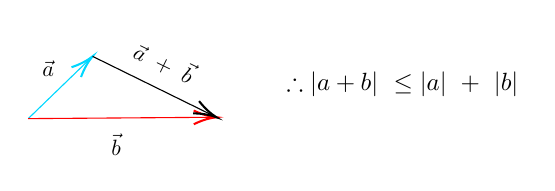
\begin{tikzpicture}[x=0.75pt,y=0.75pt,yscale=-1,xscale=1]
%uncomment if require: \path (0,300); %set diagram left start at 0, and has height of 300

%Straight Lines [id:da258083574851125] 
\draw [color={rgb, 255:red, 0; green, 215; blue, 255 }  ,draw opacity=1 ]   (98.56,121.39) -- (69,150) ;

\draw [shift={(100,120)}, rotate = 135.94] [color={rgb, 255:red, 0; green, 215; blue, 255 }  ,draw opacity=1 ][line width=0.75]    (10.93,-3.29) .. controls (6.95,-1.4) and (3.31,-0.3) .. (0,0) .. controls (3.31,0.3) and (6.95,1.4) .. (10.93,3.29)   ;
%Straight Lines [id:da4316448443334757] 
\draw [color={rgb, 255:red, 255; green, 0; blue, 0 }  ,draw opacity=1 ]   (69,150) -- (157.67,149.35) ;
\draw [shift={(159.67,149.33)}, rotate = 539.5799999999999] [color={rgb, 255:red, 255; green, 0; blue, 0 }  ,draw opacity=1 ][line width=0.75]    (10.93,-3.29) .. controls (6.95,-1.4) and (3.31,-0.3) .. (0,0) .. controls (3.31,0.3) and (6.95,1.4) .. (10.93,3.29)   ;

%Straight Lines [id:da42597634466393597] 
\draw    (100,120) -- (157.87,148.45) ;
\draw [shift={(159.67,149.33)}, rotate = 206.18] [color={rgb, 255:red, 0; green, 0; blue, 0 }  ][line width=0.75]    (10.93,-3.29) .. controls (6.95,-1.4) and (3.31,-0.3) .. (0,0) .. controls (3.31,0.3) and (6.95,1.4) .. (10.93,3.29)   ;


% Text Node
\draw (78.67,125.67) node [scale=0.8]  {$\vec{a}$};
% Text Node
\draw (134.67,122.67) node [scale=0.8,rotate=-25.96]  {$\vec{a} \ +\ \vec{b}$};
% Text Node
\draw (111.33,162.33) node [scale=0.8]  {$\vec{b}$};
% Text Node
\draw (249.33,133.33) node [scale=0.9]  {$\therefore |a+b|\ \leq |a|\ +\ |b|$};


\end{tikzpicture}
\end{center}
            
            \begin{proof}
                Method 1: Consider the cases.
                \begin{enumerate}
                    \item \(a,b \geq 0\). Then as \(a+b = \text{positive}\, \; |a+b| = a+b = |a| + |b|\)
                    \item \(a,b \leq 0\). Then \(|a+b| = |-(a+b)| = a+b = |a| + |b|\).
                    \item \(a > 0, b < 0\). Then \(|a+b| = |a-b|\), and as for the RHS, \(|a| + |-b| = |a| + |b|\). Thus as the sum of two positives is greater than the difference... Get back to this definition... \(|a+b| < |a|+|b|\).
                    \item \(a < 0, b > 0\). Then the approach is analogous to case 3.
                \end{enumerate}
                Method 2: Observe that \(|a+b|^2 = (a+b)^2 = a^2 + b^2 + 2ab\). Therefore
                \[a^2 + b^2 + 2ab \leq |a|^2 + |b|^2 + 2|a||b|\]
                \[(a+b)^2 \leq (|a| + |b|)^2\]
                Implying \(|a+b| < |a| + |b|\)
            \end{proof}
\newpage

    \begin{center}
    \fbox{\begin{minipage}{7in}
    \begin{theorem}
    A limit is unique if \(lim_{n\rightarrow \infty} a_n = a\) and $\dlim_{n\to\infty} a_n = b$. Then $a=b$.
    \end{theorem}
    \end{minipage}}
    \end{center}  
 
\tikzset{
    pattern size/.store in=\mcSize, 
    pattern size = 5pt,
    pattern thickness/.store in=\mcThickness, 
    pattern thickness = 0.3pt,
    pattern radius/.store in=\mcRadius, 
    pattern radius = 1pt}
    \makeatletter
    \pgfutil@ifundefined{pgf@pattern@name@_buu5j7212}{
    \pgfdeclarepatternformonly[\mcThickness,\mcSize]{_buu5j7212}
    {\pgfqpoint{0pt}{0pt}}
    {\pgfpoint{\mcSize+\mcThickness}{\mcSize+\mcThickness}}
    {\pgfpoint{\mcSize}{\mcSize}}
    {
    \pgfsetcolor{\tikz@pattern@color}
    \pgfsetlinewidth{\mcThickness}
    \pgfpathmoveto{\pgfqpoint{0pt}{0pt}}
    \pgfpathlineto{\pgfpoint{\mcSize+\mcThickness}{\mcSize+\mcThickness}}
    \pgfusepath{stroke}
    }}
    \makeatother
    
    % Pattern Info
     
    \tikzset{
    pattern size/.store in=\mcSize, 
    pattern size = 5pt,
    pattern thickness/.store in=\mcThickness, 
    pattern thickness = 0.3pt,
    pattern radius/.store in=\mcRadius, 
    pattern radius = 1pt}
    \makeatletter
    \pgfutil@ifundefined{pgf@pattern@name@_lw432be39}{
    \pgfdeclarepatternformonly[\mcThickness,\mcSize]{_lw432be39}
    {\pgfqpoint{0pt}{0pt}}
    {\pgfpoint{\mcSize+\mcThickness}{\mcSize+\mcThickness}}
    {\pgfpoint{\mcSize}{\mcSize}}
    {
    \pgfsetcolor{\tikz@pattern@color}
    \pgfsetlinewidth{\mcThickness}
    \pgfpathmoveto{\pgfqpoint{0pt}{0pt}}
    \pgfpathlineto{\pgfpoint{\mcSize+\mcThickness}{\mcSize+\mcThickness}}
    \pgfusepath{stroke}
    }}
    \makeatother
    \tikzset{every picture/.style={line width=0.75pt}} %set default line width to 0.75pt        
    
    \begin{tikzpicture}[x=0.75pt,y=0.75pt,yscale=-1,xscale=1]
    %uncomment if require: \path (0,300); %set diagram left start at 0, and has height of 300
    
    %Shape: Axis 2D [id:dp7674466601410441] 
    \draw  (50,248) -- (607.5,248)(69.5,63) -- (69.5,261) (600.5,243) -- (607.5,248) -- (600.5,253) (64.5,70) -- (69.5,63) -- (74.5,70) (139.5,243) -- (139.5,253)(209.5,243) -- (209.5,253)(279.5,243) -- (279.5,253)(349.5,243) -- (349.5,253)(419.5,243) -- (419.5,253)(489.5,243) -- (489.5,253)(559.5,243) -- (559.5,253)(64.5,178) -- (74.5,178)(64.5,108) -- (74.5,108) ;
    \draw   (146.5,260) node[anchor=east, scale=0.75]{1} (216.5,260) node[anchor=east, scale=0.75]{2} (286.5,260) node[anchor=east, scale=0.75]{3} (356.5,260) node[anchor=east, scale=0.75]{4} (426.5,260) node[anchor=east, scale=0.75]{5} (496.5,260) node[anchor=east, scale=0.75]{6} (566.5,260) node[anchor=east, scale=0.75]{7} (66.5,178) node[anchor=east, scale=0.75]{1} (66.5,108) node[anchor=east, scale=0.75]{2} ;
    \draw   (136,174.89) -- (142.67,181.56)(142.67,174.89) -- (136,181.56) ;
    \draw   (207,104.89) -- (213.67,111.56)(213.67,104.89) -- (207,111.56) ;
    \draw   (277,174.89) -- (283.67,181.56)(283.67,174.89) -- (277,181.56) ;
    \draw   (347,104.89) -- (353.67,111.56)(353.67,104.89) -- (347,111.56) ;
    \draw   (417,174.89) -- (423.67,181.56)(423.67,174.89) -- (417,181.56) ;
    \draw   (487,104.89) -- (493.67,111.56)(493.67,104.89) -- (487,111.56) ;
    %Straight Lines [id:da32085488103760285] 
    \draw [color={rgb, 255:red, 255; green, 0; blue, 0 }  ,draw opacity=1 ] [dash pattern={on 0.84pt off 2.51pt}]  (69.96,108.21) -- (592.82,108.21) ;
    
    
    %Straight Lines [id:da28185356751206836] 
    \draw [color={rgb, 255:red, 255; green, 0; blue, 0 }  ,draw opacity=1 ] [dash pattern={on 0.84pt off 2.51pt}]  (68.96,178.21) -- (591.82,178.21) ;
    
    
    %Straight Lines [id:da01703636370387618] 
    \draw [color={rgb, 255:red, 255; green, 0; blue, 0 }  ,draw opacity=1 ] [dash pattern={on 0.84pt off 2.51pt}]  (210.5,108) -- (209.5,247.67) ;
    
    
    %Straight Lines [id:da6121219417343098] 
    \draw [color={rgb, 255:red, 255; green, 0; blue, 0 }  ,draw opacity=1 ] [dash pattern={on 0.84pt off 2.51pt}]  (350.38,108.5) -- (349.88,247.5) ;
    
    
    %Straight Lines [id:da8026976380935107] 
    \draw [color={rgb, 255:red, 255; green, 0; blue, 0 }  ,draw opacity=1 ] [dash pattern={on 0.84pt off 2.51pt}]  (139.5,178.05) -- (139.5,247.67) ;
    
    
    %Straight Lines [id:da33319553787984724] 
    \draw [color={rgb, 255:red, 255; green, 0; blue, 0 }  ,draw opacity=1 ] [dash pattern={on 0.84pt off 2.51pt}]  (279.5,178.05) -- (279.5,247.67) ;
    
    
    %Straight Lines [id:da14615773470614601] 
    \draw [color={rgb, 255:red, 255; green, 0; blue, 0 }  ,draw opacity=1 ] [dash pattern={on 0.84pt off 2.51pt}]  (419.5,178.05) -- (419.5,247.67) ;
    
    
    %Straight Lines [id:da23101223182095065] 
    \draw [color={rgb, 255:red, 255; green, 0; blue, 0 }  ,draw opacity=1 ] [dash pattern={on 0.84pt off 2.51pt}]  (490.38,108.5) -- (489.88,247.5) ;
    
    
    %Shape: Ellipse [id:dp2825994816124451] 
    \draw  [color={rgb, 255:red, 255; green, 3; blue, 3 }  ,draw opacity=1 ][pattern=_buu5j7212,pattern size=6pt,pattern thickness=0.75pt,pattern radius=0pt, pattern color={rgb, 255:red, 247; green, 0; blue, 0}] (69.36,161.21) .. controls (73.12,161.21) and (76.17,168.82) .. (76.17,178.21) .. controls (76.17,187.61) and (73.12,195.22) .. (69.36,195.22) .. controls (65.61,195.22) and (62.56,187.61) .. (62.56,178.21) .. controls (62.56,168.82) and (65.61,161.21) .. (69.36,161.21) -- cycle ;
    %Shape: Ellipse [id:dp5133650750194041] 
    \draw  [color={rgb, 255:red, 255; green, 3; blue, 3 }  ,draw opacity=1 ][pattern=_lw432be39,pattern size=6pt,pattern thickness=0.75pt,pattern radius=0pt, pattern color={rgb, 255:red, 247; green, 0; blue, 0}] (69.96,91.21) .. controls (73.72,91.21) and (76.77,98.82) .. (76.77,108.21) .. controls (76.77,117.61) and (73.72,125.22) .. (69.96,125.22) .. controls (66.21,125.22) and (63.16,117.61) .. (63.16,108.21) .. controls (63.16,98.82) and (66.21,91.21) .. (69.96,91.21) -- cycle ;
    
    % Text Node
    \draw (139.5,185.5) node [scale=0.8]  {$a_{1}$};
    % Text Node
    \draw (210.5,116.5) node [scale=0.8]  {$a_{2}$};
    % Text Node
    \draw (280.5,186.9) node [scale=0.8]  {$a_{3}$};
    % Text Node
    \draw (350.5,116.9) node [scale=0.8]  {$a_{4}$};
    % Text Node
    \draw (420.5,186.9) node [scale=0.8]  {$a_{5}$};
    % Text Node
    \draw (490.5,116.9) node [scale=0.8]  {$a_{6}$};
    \end{tikzpicture}   
    \begin{proof}
                Fix \(\varepsilon>0\). Since the \(\dlim_{n\rightarrow \infty} a_n = a\), there exists \(N_1 \in \mathbb{N}\) s.t if \(n\geq N_1\) then \(|a_n - a| < \frac{\varepsilon}{2}\). Since the limit \(\dlim_{n\rightarrow \infty} a_n = b\),
                there exists \(N_2 \in \mathbb{N}\) s.t if \(n\geq N_2\), then \(|a_n - b| < \frac{\varepsilon}{2}\). Now if \(n\geq \text{max}\{N_1,N_2\}\). Then
                \[|a-b| = |(a-a_n) + (b-a_n)|\]
                \[\leq |a-a_n| + |b-a_n|\]
                \[< \frac{\varepsilon}{2} + \frac{\varepsilon}{2} = \varepsilon\]
                This holds for any \(\varepsilon>0\) therefore \(|a-b| = 0\) and thus \(a = b\).

            \end{proof}

	    \begin{center}
	    \fbox{\begin{minipage}{7in}
		\begin{theorem}[Squeeze Theorem]
	    Suppose you have \((a_n)_{n=1}^\infty , (b_n)_{n=1}^\infty , (c_n)_{n=1}^\infty\) are such that
            \begin{enumerate}
                \item \(a_n \leq b_n \leq c_n, \; \forall n\in \mathbb{N}\)
                \item \(\dlim_{n\rightarrow \infty} a_n = \dlim_{n\rightarrow \infty} c_n = L\). 
            \end{enumerate}
	    Then \(\dlim_{n\rightarrow \infty} b_n = L\).
	    \end{theorem}
	    \end{minipage}}
	    \end{center}
                        %UP TO DATE as of 5/03/19 evening.

            \begin{proof}
                Observe that \[|b_n - L| = |(b_n -a_n) + (a_n - L)|\]
                \[\leq |b_n - a_n| + |a_n - L| = (b_n - a_n) + |a_n - L|\]
                \[\leq (c_n - L) + |a_n -L| = |(c_n - L) + (L-a_n)| + |a_n - L| \]
                Fix \(\varepsilon > 0\). There exists \(N_1 \in \mathbb{N}\)
		such that if \(n \geq N_1\). Then there also exists some cutoff
		point \(N_2 \in \mathbb{N}\) such that if \(n \geq N_2\) then \(|c_n - L| < \frac{\varepsilon}{3}\).
                Set \(N = \text{max}\{N_1,N_2\}\). If \(n\geq N\) then
                \[b_n - L \leq |c_n - L| + 2|a_n-L|\]
                \[b_n - L \leq \frac{\varepsilon}{3} + 2\frac{\varepsilon}{3} = \varepsilon\]
                Thus \(\dlim_{n\to\infty} b_n = L\)
            \end{proof}

	    \begin{example}
	    Find \[\lim_{n\rightarrow \infty} \frac{|\sin (n^2 + 1)|}{n^2}\]
            Define that \(a_n = 0 \forall n\in\mathbb{N}\). Define \(c_n = \frac{1}{n} \forall n \in \mathbb{N}\). We know that \(|\sin(x)| \leq 1 \forall x \in \mathbb{R}\).
            \[0 = a_n \leq \frac{|\sin(n^2+a)|}{n^2} \leq \frac{1}{n^2} \leq \frac{1}{n} = c_n\]
            Clearly, \(\dlim_{n\rightarrow \infty} a_n = 0\). The claim is that
	    \(\dlim_{n\to\infty} c_n = \lim_{n\to\infty} \frac{1}{n} = 0\).
            Indeed, take \(\varepsilon > 0\). Observe that \(|c_n - 0| = c_n
	    = \frac{1}{n}\). Then \(\frac{1}{n} < \varepsilon\) if and only if \(n>\frac{1}{\varepsilon}\)
            which happens if \(n \geq [\frac{1}{\varepsilon}] + 100\). If we set \(N = [\frac{1}{\varepsilon}] + 100\), then \(n\geq N\), then \(\frac{1}{n} < \varepsilon \). Thus \(\dlim_{n\to\infty}c_n = 0\).
            \[\lim_{n\to\infty} c_n = \lim_{n\to\infty} a_n = 0\]
            \[\frac{|\sin(n^2 + 1)|}{n^2} = 0\]
	    \end{example}
            \begin{proof}
                Assume \(\dlim_{n\to\infty} a_n = L \in \mathbb{R}\). Take \(\varepsilon = 1\). There exists some \(N \in \mathbb{N}\) s.t. if \(n \geq N\), then \(|a_n - L| < 1 \). The second triangle inequality implies:
                \[||x| - |y|| \leq ||x-y||\]
                \(|a_n| - |L| \leq 1 \), which clearly implies that
		\(|a_n|<|L|+1\). Remember, \(n\geq N\), however is not a problem. Define \(M = max{|L| + 1, |a_1|, |a_2|, ... |a_{n-1}|, |a_n|}\). Obviously, 
                \(a_n \leq M \; \forall n\in \mathbb{N}\)
            \end{proof}


	\begin{center}
	\fbox{\begin{minipage}{7in}
	    \begin{theorem}
	 Assume \(\dlim_{n\to\infty} a_n = a , \dlim_{n\to\infty} b_n = b\). Fix \(\lambda \in \mathbb{R}\). Then,
        \begin{enumerate}
            \item \(\dlim_{n\to\infty} (a_n + b_n) = a+b\)
            \item \(\dlim_{n\to\infty} \lambda a_n = \lambda a\)
            \item \(\dlim_{n\to\infty}a_n b_n = ab\)
            \item \(\dlim_{n\to\infty} \frac{a_n}{b_n} = \frac{a}{b}\) if \(b_n \neq 0\) for \(n\in \mathbb{N}\) and \(b \neq 0\).
        \end{enumerate}
	    \end{theorem}
	\end{minipage}}
	\end{center}  
                Corallary: \(\dlim_{n\to\infty} (a_n - b_n) = a-b\). This is proved by both 1 and 2, if you set \(\lambda = -1\).\\
        \begin{proof}
            1 and 2: Left as an exercise to the reader... \\
        \end{proof}
        \begin{proof}
                3. \(\dlim_{n\to\infty} a_n b_n = ab \forall n\in \mathbb{N}\) and \(b\neq 0\). Therefore \(|a_n b_n - ab| < \varepsilon\).
            \begin{align*}
                &=|(a_n b_n - a_n b) + (a_n b - ab)|\\
                &=|a_n(b_n - b) + b(a_n - a)|\\
                &\leq |a_n||b_n - b| + |b||a_n-a|\\
            \end{align*}

            
            As \(|a_n|\) converges, Eg. \(|a_n| < M|b_n - b| + |b||a_n - a|\). Fix \(\varepsilon > 0\). There exists \(N_1 \in \mathbb{N}\) s.t. if \(n \geq N_1\). Thus,
            \(|b_n - b| < \frac{\varepsilon}{2M}\). Also, there exists \(N_2 \in \mathbb{N}\) s.t. if \(n \geq N_2\) then \(|a_n - a| \leq \frac{\varepsilon}{2|b|}\)
            \begin{align*}
            |a_n b_n - ab| &= M|b_n - b| + |b||a_n - a| < \varepsilon \\
            M \cdot \frac{\varepsilon}{2M} + |b| \cdot \frac{\varepsilon}{2|b|} &= \frac{\varepsilon}{2} + \frac{\varepsilon}{2} = \varepsilon 
            \end{align*}
            
            
            

        \end{proof}

        \begin{proof}
            4. Take 1 and 2 as 
        \end{proof}

        \subsection{Examples of Limits}
        Show that \[\lim_{n\to\infty} \frac{n-1}{n^3 +6} = 0\]

        Observer that \(\frac{n-1}{n^3+6} \geq 0\).
        \[\frac{n-1}{n^3 + 6} \leq \frac{n}{n^3+6} \leq \frac{n}{n^3} = \frac{1}{n^2} \leq \frac{1}{n}\]
        Thus, using the Squeeze Theorem.
        \[0 \leq \frac{n-1}{n^3 +6} \leq \frac{1}{n}\]
        Taking limits we find:
        \[
            \lim_{n\to\infty} \frac{n-1}{n^3 +6} = 0
        \]

	\begin{center}
	\fbox{\begin{minipage}{7in}
	\begin{theorem}[Convergent Sequences are bounded]
	More precisely, if \((a_n)_{n=1}^\infty\) converges, then
        \[
            \exists M > 0 : |a_n| \leq M \;\forall n \in \mathbb{N}
        \]
	\end{theorem}
	\end{minipage}}
	\end{center}
	                \begin{proof}
            Let us first show that
            \[
                \lim_{n\to\infty} \frac{1}{b_n} = \frac{1}{b}\]
            Fixing \(\varepsilon > 0\) thus,
	    \begin{align*}    
	      \left|\frac{1}{b_n} - \frac{1}{b}\right| &< \varepsilon\\
	      \frac{b-b_n}{b\cdot b_n} &< \varepsilon\\
	    \frac{|b_n - b|}{|b||b_n|} &< \varepsilon
	    \end{align*}
            
            We need to show that \(|b_n|\) does not get "too small". We know that \(\dlim_{n\to\infty} b_n = b \neq 0\). Use the def. of the limit with \(\varepsilon = \frac{|b|}{2}\).
            \[\exists \; N_1 \in \mathbb{N} : n > N_1, |b_n - b| < \frac{|b|}{2}\]
            Now we need to show that \(|b_n|\) does not get smaller. Using the Second Triangle Inequality:
            \[
                ||b_n| - |b|| \leq |b_n - b|\]
            \[
                |b| - |b_n| \leq |b - b_n| < \frac{|b|}{2}\]
            Which implies that,
            \[
                |b| - |b_n| < \frac{|b|}{2}\]
            Thus we can manipulate the inequality such that,
            \[
                |b| \leq \frac{|b|}{2} + |b_n|\]
            \[
                |b| - \frac{|b|}{2} \leq |b_n|\]
            \[
                |b_n| \geq |b| - \frac{|b|}{2}\]
            \[
                \therefore |b_n| \geq \frac{|b|}{2} > 0\]
            Now we can show that,
            \[
                |\frac{1}{b_n} - \frac{1}{b}| \leq \frac{|b - b_n|}{|b||b_n|} \leq  \frac{|b - b_n|}{|b| \cdot \frac{|b|}{2}}\]
            \[
                = \frac{2|b-b_n|}{|b|^2}\]
                
        \end{proof}
	\begin{remark}
	\begin{enumerate}
                \item If \(\lambda \in (-1,1)\) then, \[\lim_{n\to\infty} \lambda^n = 0\]
                \item Given \(c > 0\), \[\lim_{n\to\infty} c^{\frac{1}{n}} = \lim_{n\to\infty} \sqrt[n]{c} = 1\]
                \item \[\lim_{n\to\infty} n^{\frac{1}{n}} = 1\]
            \end{enumerate} 
	\end{remark}

	\begin{center}
	\fbox{\begin{minipage}{7in}
	\begin{definition}
	The sequence $(a_n)_{n = 1}^\infty$ is 'monotone increasing' if every term 'a' is bigger than the next (if $a_{n+1} \geq a_n$). Monotone decreasing is defined analogously \((a_{n+1} < a_n)\). Generally it is defined as monotone if it is either monotone decreasing or increasing.
	\end{definition}
	\end{minipage}}
	\end{center}
	
	\begin{remark}
	Sometimes the terms non-increasing, non-decreasing, strictly increasing, stricly decreasing are used.
	\end{remark}

	\begin{center}
	\fbox{\begin{minipage}{7in}
	    \begin{theorem}[Convergence of a monotone sequence]
          A monotone sequence converges if and only if it is bounded.
	\end{theorem}
	\end{minipage}}
	\end{center}
            

\tikzset{every picture/.style={line width=0.75pt}} %set default line width to 0.75pt        

\begin{tikzpicture}[x=0.75pt,y=0.75pt,yscale=-1,xscale=1]
%uncomment if require: \path (0,300); %set diagram left start at 0, and has height of 300

%Shape: Axis 2D [id:dp31358655466825613] 
\draw  (46,240) -- (600.5,240)(89.5,66) -- (89.5,257) (593.5,235) -- (600.5,240) -- (593.5,245) (84.5,73) -- (89.5,66) -- (94.5,73) (121.5,235) -- (121.5,245)(153.5,235) -- (153.5,245)(185.5,235) -- (185.5,245)(217.5,235) -- (217.5,245)(249.5,235) -- (249.5,245)(281.5,235) -- (281.5,245)(313.5,235) -- (313.5,245)(345.5,235) -- (345.5,245)(377.5,235) -- (377.5,245)(409.5,235) -- (409.5,245)(441.5,235) -- (441.5,245)(473.5,235) -- (473.5,245)(505.5,235) -- (505.5,245)(537.5,235) -- (537.5,245)(569.5,235) -- (569.5,245)(57.5,235) -- (57.5,245)(84.5,208) -- (94.5,208)(84.5,176) -- (94.5,176)(84.5,144) -- (94.5,144)(84.5,112) -- (94.5,112) ;
\draw   (128.5,252) node[anchor=east, scale=0.75]{1} (160.5,252) node[anchor=east, scale=0.75]{2} (192.5,252) node[anchor=east, scale=0.75]{3} (224.5,252) node[anchor=east, scale=0.75]{4} (256.5,252) node[anchor=east, scale=0.75]{5} (288.5,252) node[anchor=east, scale=0.75]{6} (320.5,252) node[anchor=east, scale=0.75]{7} (352.5,252) node[anchor=east, scale=0.75]{8} (384.5,252) node[anchor=east, scale=0.75]{9} (416.5,252) node[anchor=east, scale=0.75]{10} (448.5,252) node[anchor=east, scale=0.75]{11} (480.5,252) node[anchor=east, scale=0.75]{12} (512.5,252) node[anchor=east, scale=0.75]{13} (544.5,252) node[anchor=east, scale=0.75]{14} (576.5,252) node[anchor=east, scale=0.75]{15} (64.5,252) node[anchor=east, scale=0.75]{-1} (86.5,208) node[anchor=east, scale=0.75]{1} (86.5,176) node[anchor=east, scale=0.75]{2} (86.5,144) node[anchor=east, scale=0.75]{3} (86.5,112) node[anchor=east, scale=0.75]{4} ;
%Straight Lines [id:da8926008003565098] 
\draw [color={rgb, 255:red, 255; green, 0; blue, 0 }  ,draw opacity=1 ]   (90.5,112) -- (617.5,112) ;
\draw [shift={(619.5,112)}, rotate = 180] [color={rgb, 255:red, 255; green, 0; blue, 0 }  ,draw opacity=1 ][line width=0.75]    (10.93,-3.29) .. controls (6.95,-1.4) and (3.31,-0.3) .. (0,0) .. controls (3.31,0.3) and (6.95,1.4) .. (10.93,3.29)   ;

%Straight Lines [id:da21024388837811658] 
\draw [color={rgb, 255:red, 255; green, 0; blue, 0 }  ,draw opacity=1 ]   (89.5,175) -- (616.5,175) ;
\draw [shift={(618.5,175)}, rotate = 180] [color={rgb, 255:red, 255; green, 0; blue, 0 }  ,draw opacity=1 ][line width=0.75]    (10.93,-3.29) .. controls (6.95,-1.4) and (3.31,-0.3) .. (0,0) .. controls (3.31,0.3) and (6.95,1.4) .. (10.93,3.29)   ;


% Text Node
\draw (122,210) node   {$a_{1}$};
% Text Node
\draw (154,197) node   {$a_{2}$};
% Text Node
\draw (183,184) node   {$a_{3}$};
% Text Node
\draw (217,171) node   {$a_{4}$};
% Text Node
\draw (250,155) node   {$a_{5}$};
% Text Node
\draw (282,144) node   {$a_{6}$};
% Text Node
\draw (315,138) node   {$a_{7}$};
% Text Node
\draw (345,145) node   {$a_{8}$};
% Text Node
\draw (373,136) node   {$a_{7}$};
% Text Node
\draw (598,90) node   {$\mathrm{Bounds}$};
% Connection
\draw    (132.5,205.73) -- (141.65,202.02) ;
\draw [shift={(143.5,201.27)}, rotate = 517.89] [color={rgb, 255:red, 0; green, 0; blue, 0 }  ][line width=0.75]    (10.93,-3.29) .. controls (6.95,-1.4) and (3.31,-0.3) .. (0,0) .. controls (3.31,0.3) and (6.95,1.4) .. (10.93,3.29)   ;


\end{tikzpicture}

            \begin{proof}
                \(\Rightarrow \) Already done in question.\\
                \(\Leftarrow \) Assume \((a_n)_{n=1}^\infty \) is increasing. Define 
                \[
                    \alpha = \sup \{a_1, a_2, a_3 ...\} \]
                    Since \((a_n)_{n=1}^\infty\) is bounded, then the \(\sup\) exist. By another theorem, given \(\varepsilon > 0, \; \exists N \in \mathbb{N} : a_n \in (a - \varepsilon] \).
            \end{proof}

	    \begin{center}
	    \fbox{\begin{minipage}{7in}
	    \begin{definition}
	    Given \((a_n)_{n=1}^\infty\), define \[x_n = \sup\{a_n, a_{n+1}, a_{n+2} ...\} \text{ and } y_n = \sup \{a_n, a_{n+1}, a_{n+2} ... \}\] 

	    The number \( \(\dlim_{n\to\infty} x_n\) is called the upper limit
	    of (ok boomer)
	    %Need to update this... lol. 
	    Similarly, we define the no. \( \(\dlim_{n\to\infty} y_n\) is the lower limit of \((a_n)_{n=1}^\infty\), written \( \(\dlim_{n\to\infty} \inf a_n\)

	    \end{definition}
	    \end{minipage}}
	    \end{center}

	    \begin{note}
	    \(\dlim_{n\to\infty} \sup a_n\) can be \(\infty \) and \( \(\dlim_{n\to\infty} \inf a_n \) can be \(-\infty\) 
	    \end{note}
	    	    \begin{center}
	    \fbox{\begin{minipage}{7in}
	    \begin{theorem}
	    Consider sequences \((a_n)_{n=1}^\infty\) and \((b_n)_{n=1}^\infty\) given by \(a_n = (a+ 
	    \frac{1}{n})^n, b_n = (1+ \frac{1}{n})^n , n \in \mathbb{N}\). Then \((a_n)_{n=1}^\infty\) is monotone increasing and \((b_n)_{n=1}^\infty\) is decreasing, and \( \lim_{n \to \infty} a_n = \lim_{n \to \infty} b_n \)
	    \end{theorem}
	    \end{minipage}}
	    \end{center}
	    	    %A large chunk of lectures need to be filled from here
	    
	    
	    \chapter{Functions}
	    \section{Lemma: Bernoulli Inequality}
	    If \(x > -1\) and \(n \in \mathbb{N} \cup \{0\},\), then \((1+x)^n \geq 1+nx\)
	    We assume \(x = -1\) and \(n =0\) do not hold simultaneously
		\newpage

	    \begin{proof}
		    Fix \(\varepsilon > 0\). We need to find such that if \(0 < |x-a| < \delta\), then \(|f(x)g(x) - \ell m < \varepsilon\). Observe that
		    \begin{align*}
		      |f(x)g(x) - \ell m| &= |f(x)g(x) - f(x)m + f(x)m - \ell
		    m|\\
					  &\leq |f(x)||g(x) - m| + |m||f(x) - \ell|
		    \end{align*}
		    As \(f(x)\) converges to \(\ell, \exists \delta_1 > 0 : \) if \(0 < |x-a| < \delta_1\), then \(|f(x) - \ell| < 1\) (definition of limit with \(\varepsilon = 1\)). In this case, \(|(f(x) - \ell| < 1\) and \(|f(x)| < 1 + |\ell|\). Thus, if \(0<|x-a|< \delta_1\) then \(|f(x)g(x) - m\ell \leq (1+|\ell|)(|g(x) - m|) + |m||f(x) - \ell| \). \(\exists \delta_2 > 0 : \) if \(0 \leq |x-a| \leq \delta_2\), then \[|g(x) - m| < \frac{\varepsilon}{2(1+|\ell|)}\] Also \(\exists \delta_3 > 0 :\) if \(0 \leq |x-a| \leq \delta_3\), then \[|f(x) - \ell| < \frac{\varepsilon}{2(|m| + 1)}\] Set \(\delta = \min\{\delta_1, \delta_2, \delta_3\}\). If \(0 < |x-a| < \delta\), then
		    \begin{align*}
		      f(x)g(x) - \ell m| &\leq |1+ |\ell||g(x) - m| + |m||f(x)
		      -\ell|\\
		      &< \frac{\varepsilon}{2((1+|\ell|)} \cdot (1+|\ell|)
		      + \frac{\varepsilon}{2(|m|+1)} \cdot |m|\\
		      &< \frac{\varepsilon}{2} + \frac{\varepsilon}{2} = \varepsilon
		    \end{align*}
	    \end{proof}

	    \begin{center}
	    \fbox{\begin{minipage}{7in}
	    \begin{definition}
	    \( \(\dlim_{x\to\infty} f(x) = \ell\) if \(\forall \varepsilon > 0, \exists M > 0 : \) if \(x>M,\) then \(|f(x)- \ell| < \varepsilon\). Similarly, you can define the limit \( \(\dlim_{x\to-  \infty} f(x) = \ell\) (Reversed Definition)
	    \end{definition}
	    \end{minipage}}
	    \end{center}

	    \begin{center}
	    \fbox{\begin{minipage}{7in}
	    \begin{definition}
	    \( \dlim_{x\to a} f(x) = \infty\) if \(\forall M > 0 \exists \delta > 0 :\) if \(0<|x-a|<\delta\) then if \(f(x) > M\). Analogously, define \( \dlim_{x\to a } f(x) = -\infty, \dlim_{x\to\infty} f(x) = \infty\) etc.
	    \end{definition}
	    \end{minipage}}
	    \end{center}
	    
	    \begin{center}
	    \fbox{\begin{minipage}{7in}
	    \begin{theorem}[Squeeze Theorem]
	    Given functions \(f,g h : X \to \mathbb{R}\), if \(f(x) \leq g(x) \leq h(x) \forall x \in X, \(\dlim_{x\to a} f(x) = \(\dlim_{x\to a} h(x) = \ell\) then \( \(\dlim_{x\to a} h(x) = \ell\). 
	    \end{theorem}
	    \end{minipage}}
	    \end{center}
	    \begin{remark}
	    We allow \(a = \pm \infty\)
	    \end{remark} 
	    

	    \begin{center}
	    \fbox{\begin{minipage}{7in}
	    \begin{theorem}[Limit of Subsequences]
	    The following are equivalent:
	    \begin{enumerate}
		    \item \( \(\dlim_{x\to a} f(x) = \ell\)
		    \item \( \(\displaystyle \lim_{n\to \infty} f(x_n) = \ell\) for every sequence \( (x_n)_{n=1}^\infty\) s.t. \( \(\dlim_{x\to \infty} x_n = a\)
	    \end{enumerate}
	    \end{theorem}
	    \end{minipage}}
	    \end{center}
	    	    %Insert Graphics here

	    \begin{proof}
	      We need to prove from both sides of the equivalence, we begin by
	      proving that (1) \( \implies \) (2).
		    Assume 2) holds, but 1) does not hold. Then \( \(\dlim_{x\to a} f(x)\) does not exist or it does not equal \(\ell\). Therefore \(\exists \varepsilon_0 > 0\) s.t. \(\forall \delta > 0\), there is \(x \in \{a - \delta, a + \delta\} \setminus \{a\}\)
	    \begin{center}
	      \begin{tikzpicture}
		\draw[<->] (0,-0.2) -- (0,5);
		\draw (0,3) node [anchor=east] { \( \ell \)};
		\draw (3,0) node [anchor=south]  { \( a \) };
		\draw (0,5) node [anchor=east] {\( f(x) \)};
		\draw (8,0) node [anchor=south] { \( x \) };
		\draw[<->] (-1, 0.5) -- (8,0.5);
		\draw (-1,1) to [bend right = 20] (3,3);
		\draw[->] (3,3) to [bend left = 40] (7.5, 3.5);
		\draw[dotted] (0,3) -- (3,3);
		\draw[dotted] (3,0.5) -- (3,3);
		\draw node at (3,3)[circle, fill, inner sep=1pt];
	    \end{tikzpicture}
	    \end{center}
	    Take \( \delta = 1 \), this implies that \( \exists x_1 \in (a-1,
	    a+1)\setminus \{a\} \) such that \( |f(x_1) - \ell| \geq
	    \varepsilon_0 \). Now take \( \delta = \frac{1}{2} \implies
	    \exists x_2 \in (a- \frac{1}{2}, a+ \frac{1}{2}) \) such that \(
	    |f(x_2) - \ell| \geq \varepsilon_0 \). Setting \( \delta
	    = \frac{1}{3}, \frac{1}{4}...\) so forth, allows us to obtain
	    a sequence of \( \mathbb{R} \), \( (x_n)_{n=1}^\infty \) such that
	    \( \dlim_{n \to \infty} x_n = a\) and \( |f(x) - l| \geq
	    \varepsilon_0 \), \( \forall n \in \mathbb{N} \). Which is
	    a contraposition
	    \end{proof}

	    \section{Continuity}
	    \begin{center}
	    \fbox{\begin{minipage}{7in}
	    \begin{definition}
	    If \( X \subseteq \mathbb{R}  \), \( f:X\to \mathbb{R} \), for \(
	    a \in X \). We say that \( f \) is continuous at \( a \) if and only if
	    \[ 
	      \displaystyle \lim_{x \to a} f(x) = f(a)
	    \]
	    \end{definition}
	    \end{minipage}}
	    \end{center}

	    \begin{center}
	    \begin{tikzpicture}
	      % Grid Axis
	      \draw[->] (0,-1) -- (0,5);
	      \draw[->] (-1,0) -- (10,0);
	      \draw [grey!50] (-1,1) -- (0,1) -- (3,3)  -- (7,1.5) -- (10,4);
	      \draw[->] plot [smooth, tension = 1] coordinates { (-1,1)
		(0,1) (3,3) (7,1.5) (10,4)};
	      \draw[dotted] (3,0) -- (3,3);
	      \draw node at (3,3)[circle, fill, inner sep=1.3pt];
	      \draw (3,3) node [anchor=south] { \( f(a) \) };
	    \end{tikzpicture}
	    \end{center}

	    Alternatively, \( f \) is continuous at \( a \) if \( \forall
	    \varepsilon > 0 \), \( \exists \delta > 0 \) such that if \( |x-a|
	    < \delta \) then, \(|f(x) - f(a)| < \varepsilon \).

	    \begin{center}
	    \fbox{\begin{minipage}{7in}
	    \begin{definition}
	    We say \( f:X \to \mathbb{R} \) is continuous on \( X \subseteq
	    \mathbb{R} \) if \( f \) is continuous \( \forall x \in X \).
	    \end{definition}
	    \end{minipage}}
	    \end{center}

	    \begin{example}
	      Dumb spacing
	    \begin{enumerate}
	      \item \( f(x) = x \), is continuous on \( \mathbb{R} \).
	      \item \( f(x) = a \), is continuous on \( \mathbb{R} \).
	    \end{enumerate}
	    \end{example}

	    \begin{center}
	    \fbox{\begin{minipage}{7in}
	    \begin{theorem}
	    Assume you have 2 functions, \( f \) and \( g \), such that 
	    \[ 
	      f,g:(a,b) \to \mathbb{R}
	    \]
	    are continuous at \( x_0 \in (a,b) \) then
	    \begin{enumerate}
	      \item \( (f+g)(x) = f(x) + g(x) \) is continuous at \( x_0 \).
	      \item \( f,g \) are continuous at \( x_0 \).
	      \item \( \frac{f}{g} \) is continuous at \( x_0 \).
	    \end{enumerate}
	    \end{theorem}
	    \end{minipage}}
	    \end{center}

	    \begin{proof}
	    This follows immediately from some previous theorem I can't read
	    from my handwriting.
	    \end{proof}

	    \begin{col}
	      Every polynomial function is contnuous on \( \mathbb{R} \).
	      moreover, every function of the form \( \df{P(x)}{Q(x)} \), \(
	      P \), \( Q \), polynomial is continuous at every \( x \) such
	      that \( Q(x) \neq 0 \). Whenever \( P(x) \) and \( Q(x) \) are
	      rational functions.
	    \end{col}

	    \section{Character Building}
	    \begin{center}
	    \fbox{\begin{minipage}{7in}
		\begin{theorem}[Character Building Theorem]
		  Suppose \( f \) is continuous on a closed bounced interval \(
		  [a,b]\). Then \( f \) is uniform continuous on \( [a,b] \) on
		  \( [a,b] \) (if closed, bounded, uniform continuous \(
		  \implies \) continuous).
	    \end{theorem}
	    \end{minipage}}
	    \end{center}

	    \begin{proof}
	    By contradiction, assume that \( f \) is not uniform continuous.
	    Then \( \exists \varepsilon_0 > 0 \) such that \( \forall \delta
	    > 0 \), \( \exists x,y \in [a,b] \) with 
	    \[ 
	      |x-y| < \delta \text{ but } |f(x) - f(y)| \geq \varepsilon_0
	    \]
	    \end{proof}
	    \begin{center}
	      \begin{tikzpicture}
		% GRID AXIS
		\draw[->] (0,-1) -- (0,5);
		\draw[->] (-1,0) -- (10,0);
	      \end{tikzpicture}
	    \end{center}
	    
	    
	    
	    
\end{document}
